\section{Desarrollo}
%Deben explicarse los m´etodos num´ericos que utilizaron y su aplicaci´on al problema
%concreto involucrado en el trabajo pr´actico. Se deben mencionar los pasos que siguieron
%para implementar los algoritmos, las dificultades que fueron encontrando y la
%descripci´on de c´omo las fueron resolviendo. Explicar tambi´en c´omo fueron planteadas
%y realizadas las mediciones experimentales. Los ensayos fallidos, hip´otesis y conjeturas
%equivocadas, experimentos y m´etodos malogrados deben figurar en esta secci´on, con
%una breve explicaci´on de los motivos de estas fallas (en caso de ser conocidas).

Para resolver el sistema lineal anteriormente propuesto:
\begin{equation*}
(\textbf{I} - \textit{p } \textbf{W D}) x = \gamma \textbf{ e}
\end{equation*}
donde $\gamma = \textbf{z}^T \textbf{x}$ y suponemos $\gamma = 1$,
utilizaremos el algoritmo de Eliminaci\'on Gaussiana sin pivoteo. \\

\subsection{Implementación}
Para implementarlo, tuvimos en cuenta que la matriz que define el sistema
tiene muchos espacios en 0 en casos de la vida real, ya que la cantidad de links
que tiene una página web es pequeña en comparación con la cantidad de páginas
existentes. Es por esto que implementamos una clase de Matriz Rala o Dispersa,
que guarde solamente los elementos distintos a 0 y de esta forma ahorrar espacio y optimizar
las operaciones.

Al pensar posibles formas de representar dicha estructura, decidimos probar primero con un vector de vectores, donde cada elemento se guarda en un vector fila y este contiene su valor y su posición en la fila. Además, realizamos los algoritmos prestando atención a que cada elemento de cada fila quede ordenado por la posición de los elementos en la matriz real, de forma que podamos usar Búsqueda Binaria. La siguiente estructura que consideramos fue la de cambiar la representación de cada fila por un mapa. Terminamos usando la implementación con vectores, dado que era más eficiente en tiempo (ver sección Resultados).

Otra cosa que tuvimos en cuenta fue que la matriz \textbf{D} es diagonal, para implementar la multiplicación \textbf{W D} de forma óptima. Además, utilizamos un \textit{epsilon} de $10^{-7}$ para definir cuando un número debía ser tratado como igual a 0. Teniendo en cuenta que los tests de la cátedra debían tener a lo sumo $10^{-5}$ de error, consideramos que $10^{-7}$ es lo suficientemente grande para detectar errores numéricos pero lo suficientemente chico para no tener falsas detecciones, teniendo en cuenta que trabajamos con números pequeños.

Para facilitar la búsqueda de errores en el código, implementamos primero las
operaciones básicas de matriz (multiplicación, resta), creamos tests para estas
(utilizado el framework \textit{Google Test}), y luego pasamos a implementar
la EG, testeándola con los archivos provistos por la cátedra.

Desde un comienzo, utilizamos \textit{long double} para almacenar los elementos
de las matrices de la forma más precisa posible. Posteriormente, probamos
si realmente el uso de \textit{long double} prevenía problemas de precisión
o no, frente a \textit{double} y \textit{float}.

Dado que se nos pide normalizar el vector \textbf{x} de forma que
$\sum_{i} \textit{x}_i = 1$, dividimos a cada elemento de \textbf{x} por la
sumatoria de sus elementos. Esto lleva a problemas de precisión, dada la suma
de números que potencialmente tendrían distinta magnitud. Es por eso que
probamos con distintos métodos:
\begin{itemize}
\item Suma normal
\item Suma normal, ordenando antes los números de forma ascendente
\item Suma con algoritmo de Kahan
\end{itemize}

% \subsection{Experimentación sobre predicados teóricos}
% Sabemos que cuanto mayor sea el n\'umero de condici\'on de una matrix, mayor ser\'a su inestabilidad. 
% En otras palabras, si utilizamos dicha matriz para construir un sistema lineal, pequeños cambios en las variables 
% del sistema, producen resultados muy distintos. Esto, reflejado sobre la aplicaci\'on de nuestro algoritmo implica que, 
% si la matriz tiene un n\'umero de condici\'on muy grande entonces el resolver el sistema es propenso a errores. Ahora, 
% dado que las matrices con las que trabajamos dependen de $p$, la motivaci\'on de este experimente es ver que sucede con el 
% error a medida que $p$ crece. 

\subsection{Experimentación cuantitativa}
Empezando por la experimentación cuantitativa, creamos un script en C++ que nos
provea de la matriz \textbf{A}, aprovechando el código anteriormente implementado.
Luego, utilizamos \textit{Octave} para ver el error producido al aproxims
\textit{x'} obtenida ($|Ax' - x'| \approx 0$). Para ver el error absoluto,
volvimos a usar \textit{Octave} para ver la distancia entre nuestras soluciones
y las dadas por la cátedra.

\subsection{Experimentación cualitativa}
Para la experimentación cualitativa, primero pensamos casos no triviales de conjuntos de
páginas y links que nos parecian de interés.
Los graficamos usando una herramienta web y generamos los archivos .txt que representan cada 
uno de los casos, en el formato de entrada con el que trabaja nuestro ejecutable de C++.
Definimos experimentos usando estos casos, y para correrlos utilizamos la ayuda de \textit{Octave}.
Los resultados de cada experimento se visualizan de diferentes formas, usando gráficos de diferente
naturaleza.

Decidimos plantear las estructuras descriptas a continuación.

\subsubsection{Malla}
La estructura consiste en 4 nodos conectados todos entre sí de manera bidireccional.
Lo que esperamos con esta estructura es que el valor de \textit{p} no importe, ya que todas las páginas tienen la misma importancia en la red. Por eso, decidimos experimentar con distintos valores de \textit{p}, dispersos en el intervalo $(0, 1)$

\begin{center}
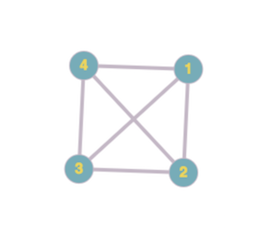
\includegraphics{malla.png}
\end{center}


\subsubsection{Página popular}
En esta estructura, todas las páginas están conectadas a una central.
Lo que esperamos es que la primer página tenga el PageRank \footnote{Siempre que calculamos el Page Rank de un sistema, a primera instancia
usamos $p = 0.65$ porque es lo suficientemente alto para descubrir las particularidades del sistema.} más alto  y que las otras páginas tengan igual ranking, pero menor. 
Aun así, esperamos que cuanto más cerca esté \textit{p} \footnote{Siempre
que graficamos rankings en función de $p$, se calcula el Page Rank para el sistema con 100 valores de $p$ distintos
espaciados de forma uniforme.} de 0, todos las páginas tiendan a tener el mismo ranking de 1/n.

\begin{center}
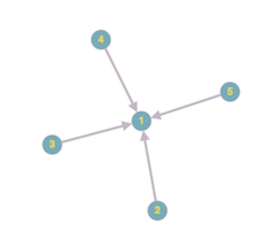
\includegraphics{pagina_popular.png}
\end{center}


\subsubsection{Escalonado}
\centerline{ \enquote{Todos los caminos conducen a Roma. (O la Página 5)} }
Esta estructura está formada por 5 nodos con la forma de una lista enlazada, de forma que la Página 5 es el final de la lista.
Lo que esperamos es que la Página 5 gane siempre el PageRank, y que la 1 siempre sea la última, ya que esta no recibe ningún link, mientras que la Página 5 está indirectamente apuntada por todas las páginas del sistema.
Además, al igual que en el caso anterior, esperamos que cuanto más cerca esté \textit{p} de 0, todas las páginas tengan el mismo ranking de 1/n.

\begin{center}
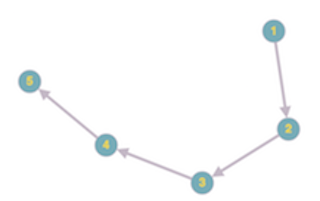
\includegraphics{escalonado.png}
\end{center}


\subsubsection{Roba éxito}
Todas la páginas tienen un link a la Página 1. Luego, las Páginas 3, 4, 5 y 6 estan contectadas entre si y la Página 1 solo tiene un link a la Página 2.
Lo que esperamos es que la Página 1 siempre tenga mayor ranking pero que sea bastante parecido al de la Página 2, ya que la primera tiene un link a la segunda. Además pretendemos que las páginas 3, 4, 5, 6 tengan el mismo ranking.
El propósito de esta estructura, es verificar un aspecto importante del algoritmo. El PageRank pretende que sea mejor recibir un solo link de una página popular, a recibir muchos links de páginas poco populares.
La idea del experimento fue corroborar que si bien la Página 2 recibe un solo link, su ranking aún así debería ser alto, dado que
que este link proviene de la Página 1, que es (o al menos esperamos que sea) la página más popular del sistema. \\

\begin{center}
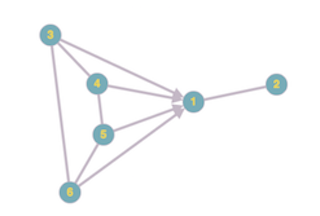
\includegraphics{roba_exito.png}
\end{center}
